In questo capitolo descriveremo le componenti che utilizzeremo nella nostra
architettura e, per ognuna di queste, introdurremo brevemente le caratteristiche chiave.

\section{OWL2}

L'OWL 2 Web Ontology Language, informalmente OWL 2, è un linguaggio ontologico, basato sulle
logiche descrittive o \textbf{DL}, costruito 
per il Semantic Web con un significato formale e definito in \cite{OWl2Primer}.
Le ontologie in OWL 2 vengono definite tramite la specifica di classi, proprietà, individui e valori dei dati e sono memorizzate come documenti del Semantic Web.
Queste possono essere pubblicate sul web e riferite da altre ontologie, per costruire basi di conoscenza più complesse. 
Inoltre sono spesso utilizzate assieme insieme a documenti scritti nel formato RDF, ed stesse vengono scambiate principalmente come documenti RDF.

\subsection{Semantica}
La semantica è definita \textit{formalmente}, cioè permette di scrivere \textit{Knowledge Base} sulle quali è possibile applicare inferenze in modo automatico.
OWl2 possiede due semantiche:
\begin{itemize}
	\item[] \textbf{Semantica diretta}, basata sulle Logiche Descrittive (vedi pag.\pageref{chap: DL})
		\begin{itemize}
			\item è applicabile a un frammento del linguaggio detto OWL2 DL;
			\item è sempre decidibile;
			\item ha una sintassi più ristretta. 
		\end{itemize}
	\item[] \textbf{Semantica Indiretta}, basata sui grafi RDF
		\begin{itemize}
			\item estende la semantica formale di RDF
			\item ha la massima espressività 
			\item la decibilità non è garantita
		\end{itemize}
\end{itemize}
la semantica è basata su \textbf{iff} (se e solo se) quindi:
\[ C \text{ è sottoclasse di D } \iff  \text{istanze di } C \subseteq \text{istanze di } D \]

\subsection{Caratteristiche}
Il linguaggio prevede tre componenti principali:
\begin{enumerate}
	\item \textbf{Entità}: elementi atomici usati per riferirsi ad oggetti, categorie e relazioni 
	del mondo reale; costituiscono gli assiomi\\ 
	$Lara,donna,Pietro,Sofia,essere\_fidanzati$ 
	\item \textbf{Assiomi}: affermazioni (\textit{statement}) di base espressi da un'ontologia OWL
	$Lara$ è una $donna$ | $ Pietro $ e $ Sofia $ sono $ fidanzati $
	\item \textbf{Espressioni}: combinazioni di entità che costituiscono descrizioni complesse, definite
	tramite l'utilizzo di costruttori. \\
	$ Medico $ e $ Donna $ combinate definiscono $ Donna Medico $ 
\end{enumerate}
 
Ogni file \textit{.owl} inizia con un preambolo: \label{code:preambolo}
\begin{minted}{XML} 
	Prefix(:=<http://example.com/owl/families/>)
	Prefix(otherOnt:=<http://example.org/otherOntologies/families/>)
	Prefix(xsd:=<http://www.w3.org/2001/XMLSchema#>)
	Prefix(owl:=<http://www.w3.org/2002/07/owl#>)
	Ontology(<http://example.com/owl/families>
	Import( <http://example.org/otherOntologies/families.owl> )
	....
\end{minted} 
\mint{XML}|Prefix(..)| permette di fare, sinteticamente, riferimento a elementi definiti in altre ontologie o in altri file; il prefisso più l'etichetta sono composti nell'identificatore dell'elemento di interesse, ad esempio
\mintinline{XML}{owl:Thing} diventa \mintinline{XML}{http://www.w3.org/2002/07/owl#Thing}.
\mint{XML}|Ontology(..)| Specifica l'\textbf{URI} (Uniform Resource Identifier) del file contenente l'ontologia definita.
\subsection{Sintassi e Modellazione di Base} \label{subSec: SintassiOWL}
È possibile scrivere ontologie OWL utilizzando sintassi differenti:
\begin{itemize}
	\item Functional-Style \mintinline{XML}{ClassAssertion(:Persona:Damiano)}
	\item Manchester \mintinline{XML}{Individual: Damiano}
	\item Turtle \mintinline{XML}{:Damiano rdf:type :Persona}
	\item RDF/XML \mintinline{XML}{<Persona rdf:about="Damiano">}
	\item OWL \begin{minted}{XML}
	<ClassAssertion>
	<Class IRI="Person"/>
	<NamedIndividual IRI="Damiano"/>
	</ClassAssertion>
	\end{minted}
\end{itemize}
Ed esiste una chiara equivalenza tra le varie terminologie utilizzate, vediamola:
\begin{multicols}{3}
	\textit{Ing. della conoscenza}
	\begin{itemize}
		\item Oggetti 
		\item Categorie 
		\item Relazioni
	\end{itemize}
	\textit{Description Logic}
	\begin{itemize}
		\item Costanti
		\item Predicati Unari 
		\item Predicati Binari
	\end{itemize}
    \textit{Termini OWL}
	\begin{itemize}
		\item Individui
		\item Classi 
		\item Proprietà
	\end{itemize}
\end{multicols}
Dopo queste considerazioni generali, entriamo ora nei dettagli della modellazione con OWL2.
Nei paragrafi successivi introdurremo le funzionalità essenziali per produrre una base di conoscenza. Queste saranno condite con esempi,
semplici dimostrazioni delle varie funzionalità di OWL.
Per semplicità useremo il \textit{Functional-Style}.

Ecco come si esprimono gli Assiomi: 
\begin{itemize}
	\item dichiarazioni di individuo: \mintinline{XML}{Declaration(Name Individual(:Dario))}
	\item dichiarazioni di classe: \mintinline{XML}{Declaration(Class(:Persona))}
	\item dichiarazioni di proprietà: \mintinline{XML}{Declaration(ObjectProperty(:Uomo))}
\end{itemize}
E alcune delle relazioni chiave:

\makebox[8cm]{\mintinline{XML}{ClassAssertion(:Persona :Dario))} \hfill} lega un'istanza ad una classe; \\
\makebox[8cm]{\mintinline{XML}{SubClassOf(:Persona :Uomo))} \hfill} relazione di sottoclasse ($ \sqsubseteq $); \\
\makebox[8cm]{\mintinline{XML}{EquivalentClasses(:Persona :Umano)}\hfill} equivalenza di due classi;\\
\makebox[8cm]{\mintinline{XML}{DisjointClasses(:Donna :Uomo)}\hfill} classi disgiunte.

Permette di legare due individui tramite una proprietà.
\mint{XML}{ObjectPropertyAssertion(:haMoglie :Donna :Uomo)}
\subsection{Classi complesse e implementazione di $ \sqcap,\sqcup,\exists $ e $ \forall $}
Tramite opportuni costrutti è possibile specificare classi complicate e relazionarle, 
anche grazie all'operatore di intersezione $\sqcap$ e disgiunzione $ \sqcup $.
\begin{minted}{XML}
	EquivalentClasses(:Padre
		ObjectIntersectionOf(:Uomo :Genitore))
	EquivalentClasses(:Genitore
		ObjectIntersectionOf(:Madre :Padre))
\end{minted}
Nonna è sottoclasse dell'intersezione fra \textit{Donna e Genitore}.
\begin{minted}{XML}
	SubClassOf(:Nonna 
		ObjectIntersectionOf(:Donna :Genitore))
\end{minted}
L'individuo \textit{Marco} è una \textit{Persona} (e) non \textit{Genitore}.
\begin{minted}{XML}
	ClassAssertion(
		ObjectIntersectionOf(:Persona 
			ObjectComplementOf(:Genitore))
	:Marco)
\end{minted}
Vediamo, infine, come si possano utilizzare i quantificatori $ \exists $ e $ \forall $ con qualche esempio.
La classe \textit{Genitore} è l'insieme di quegli individui che possiedono almeno un'istanza 
di \textit{Persona} che è loro Figlio; una persona è \textit{Felice} quanto tutti 
i suoi figli sono felici. Le persone che non hanno figli, vengono correttamente considerati felici.
\begin{multicols}{2}
	Quantificatore esistenziale $ \exists $
	\begin{minted}{XML}
	EquivalentClasses(
	  :Genitore
	  ObjectSomeValuesFrom
	  (:haFiglio :Persona))
	\end{minted}
	
	Quantificatore universale $ \forall $
	\begin{minted}{XML}
	EquivalentClasses(
	  :PersonaFelice
	   ObjectAllValuesFrom
	    (:haFiglio :PersonaFelice))
	\end{minted}
\end{multicols}

Questo conclude la nostra visione sintetica del linguaggio.

\subsection{OWL2 \emph{Versus} DB e considerazioni finali}
I file \textit{.owl} conservano informazioni ma nonostante ciò OWL2 \textbf{non} è un framework
per basi di dati; Nonostante parte della terminologia evochi assonanze con i \textbf{D}ata\textbf{B}ase, 
la semantica di base ha delle differenze sostanziali.

In primis l'assunzione di mondo: un fatto non contenuto in un \textbf{DB} è considerato falso (mondo chiuso) mentre nel mondo
logico viene considerato mancante (mondo aperto). In secondo luogo, classi e proprietà possono avere definizioni multiple e OWL non richiede che le uniche proprietà di un individuo siano quelle della classe a cui appartiene.
Come terzo punto, ci teniamo a sottolineare un ulteriore differenza sostanziale: con i \textbf{DB} non faccio ragionamento, non esplicito informazioni implicite, con OWL sì.
Infine ricordiamo ciò che abbiamo visto a \ref{code:preambolo} : le informazioni riguardanti un singolo individuo 
possono essere distribuite su più documenti diversi, contrariamente ad un classico database.

In conclusione vogliamo ricordare che OWL \textbf{non} è un linguaggio di programmazione, bensì
un linguaggio \textit{dichiarativo}, in grado di rappresentare della conoscenza. Diversi sono gli strumenti
a disposizione per trattare le ontologie: ragionatori automatici, API, validatori, editor e ambienti di sviluppo.
Nella sezione successiva tratteremo alcuni di questi tool che fanno parte di DbN.  

\section{Owlready2} \label{sec: OwlR2}
Lavorare direttamente con OWL è impegnativo e tedioso, ma, in nostro soccorso, arrivano le API (Application Programming Interface).
Tra le più recenti e interessanti spicca Owlready2 \cite{OwlReady}, pratica libreria \textit{ontology-oriented}, scritta in Python3. Owlready versione 2 permette un accesso trasparente alle ontologie, contrariamente alle API basate su Java.
Può caricare ontologie OWL2 come oggetti Python, modificarli, salvarli e, appoggiandosi ad  \textit{HermiT} e \textit{Pellet} (reasoner scritti in Java), eseguire veri e propri ragionamenti.
Vediamo alcune caratteristiche chiave.

\subsection{Tabella di conversione}
Se dovessimo "convertire" le formule tra Description Logics, Owlready2 e/o Protegè,
potrebbe essere di interesse la sottostante tabella.

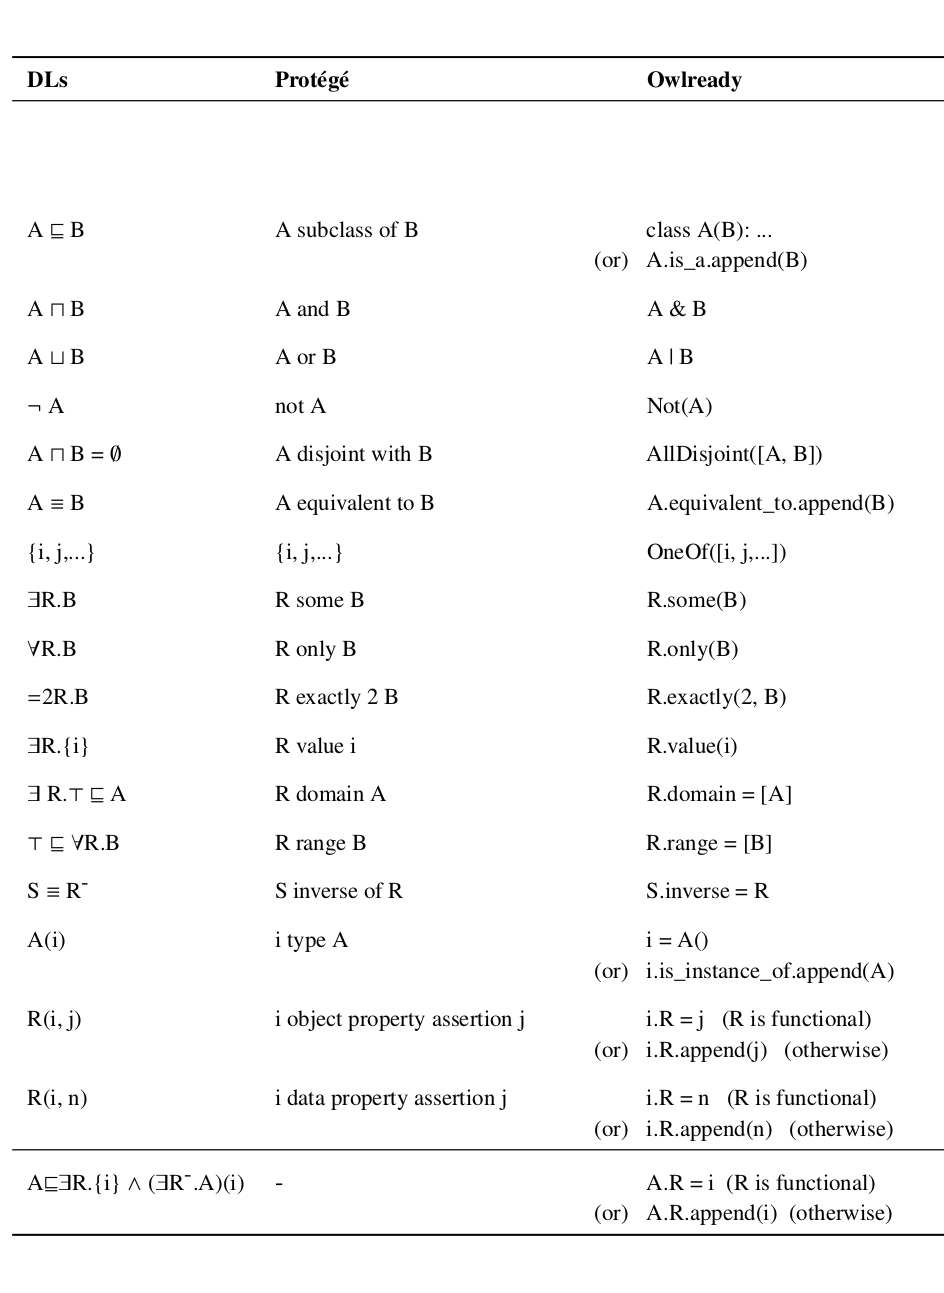
\includegraphics[width=\linewidth]{immagini/ConversionTable.png}

Molti di questi simboli ci sono familiari e, di conseguenza, 
il salto rappresentazionale è molto basso.
Utilizzare la semantica di questo pacchetto non risulta troppo impegnativo, poiché coerente
con le Logiche Descrittive.

\subsection{Che cosa posso fare con OWLReady2?}
\inputminted{Python}{codice/IntroOwlReady2.py}

\subsection{Architettura}
Le RDF Quadruple giocano un ruolo importante, diamone una definizione : 
Sia $ S $ un insieme di fonti di dati, che è un sottoinsieme del $ IRIs $ set (cioe $ S \subseteq \mathcal{I} $. Una coppia ordinata $ (t,g) $ della tripla $ t = (s,p,o) $ e del
grafo $ g \in S $ e $ t \in get(c) $ è una tripla nel grafo $ g $, dove $ get $ è una richiesta HTTP get request, e il risultato della richiesta non può essere un insieme vuoto 
($ get(s) \not = \empty $. La quadrupla $ (s,p,o,g) $ è chiamata una RDF quadrupla (RDF quad).


Owlready2 mantiene, quindi, un quadstore (\textbf{DB} di quadruple) RDF in un database ottimizzato \textit{SQLite3}, sia in memoria che, opzionalmente, su disco.\\
Fornisce, inoltre, un accesso di alto livello alle classi e agli oggetti presenti 
nell'ontologia. Classi e Individui vengono caricati dinamicamente dal \textbf{DB} secondo
necessità, salvati in memoria e poi eliminati quando non più necessari.

\subsection{Paragone con precedenti approcci}

\begin{figure}[h]
	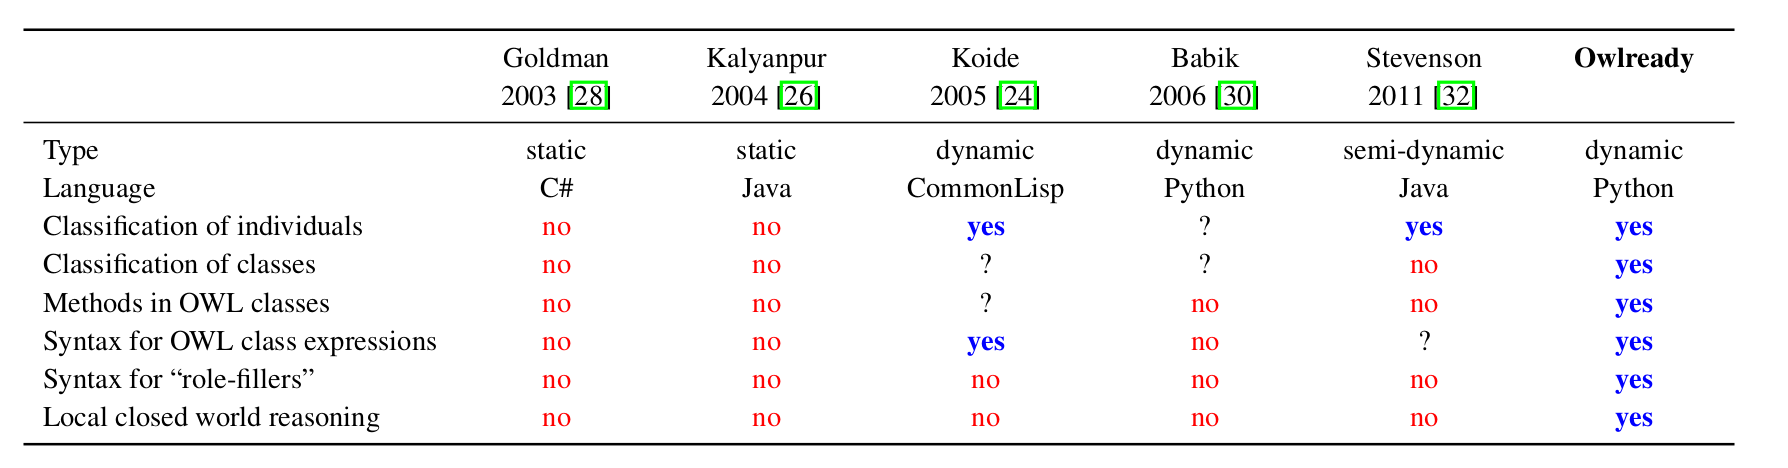
\includegraphics[width=\linewidth]{Tabella_Comp_Owlr2.png}
	\caption{Paragone di Owlready con altri approci di programmazione.}
	\centering
	\label{fig:tabComparativa}
\end{figure}

La tabella \ref{fig:tabComparativa} confronta diverse tecnologie precedenti con Owlready2.
Owlready si distingue come uno degli approcci più avanzati. In particolare,
è in grado di classificare automaticamente (non solo gli individui ma anche le classi),
compiere "reasoning" sul mondo locale chiuso e non e proporre una sintassi ad alto livello per
definire i vincoli "role-fillers". Queste ed altre caratteristiche risultano cruciali quando
si lavora utilizzando ontologie mediche, ma, certamente, non sfigurano anche in altri domini
applicativi.

Ecco, quindi, quali sono le componenti chiavi di un sistema capace di adattarsi a
differenti casi d’uso, in maniera decisamente flessibile e dinamica.

\clearpage

\section{Plotly} \label{sec: Plotly}
Plotly.py è una delle migliori librerie \textit{Open Source} di plotting: supporta oltre 40 tipi di grafici unici, 
interattivi e ricchi di funzionalità, andando a coprire una vasta gamma di casi d'uso: statistico, finanziario, geografico, 
scientifico e tridimensionale. Non mancano i classici grafici a linee, a barre, a bolle e a punti. \cite{Plotly}

\subsection{Perché usare Plotly.py?}
Costruita sopra la più celebre libreria Javascript (Plotly.js, composta da d3.js e stack.gl), 
Ploty.py permette di creare bellissime realizzazioni interattive basate sul web, che possono
essere salvate come file HTML o utilizzate come parte di web-app scritte in Python.
Tutti i grafici di Plotly.py sono completamente costumomizzabili. 
Tutto, dai colori e dalle etichette alle linee della griglia e alle legende, può essere personalizzato 
utilizzando una serie di attributi dedicati.
I diagrammi, inoltre, sono dotati di funzionalità interessanti come lo zoom, il panning, il ridimensionamento automatico, ecc. \\
Grazie all'integrazione profonda con Orca, utility per l'esportazione di immagini, Plotly.py
fornisce un notevole supporto anche per i contesti al di fuori del web, inclusi gli IDE (PyCharm, Spyder)
e la pubblicazione di documenti cartacei, come questo testo.

L'obiettivo era quello di rendere gradevoli ed esplicativi i risultati "diagnostici" prodotti dal tool DbN.

\subsection{Che cosa posso fare con Plotly.py?}
\inputminted{Python}{codice/IntroPlotly.py}






